\documentclass[11pt]{article}

% ---------------------------------------------------------------------------
% lean-primer.tex  —  A Lean 4 primer for people who prove things elsewhere.
% Source document (versioned); lean-primer.pdf is the build output.
% Build:  latexmk -pdf lean-primer.tex   (see tools/build-primer.sh)
% Engine: pdflatex + biber. Lean's Unicode is handled by listings `literate`.
% ---------------------------------------------------------------------------

\usepackage[a4paper,margin=1in]{geometry}
\usepackage[T1]{fontenc}
\usepackage{lmodern}
\usepackage{microtype}
\usepackage{amssymb,amsmath}
\usepackage{xcolor}
\usepackage{listings}
\usepackage{booktabs}
\usepackage{enumitem}
\usepackage{tikz}
\usetikzlibrary{arrows.meta,positioning,fit,backgrounds}
\usepackage[backend=biber,style=numeric,backref=true,sorting=nyt]{biblatex}
\addbibresource{refs/lean-refs.bib}
\usepackage[colorlinks=true,linkcolor=accent,citecolor=accent,urlcolor=accentdark]{hyperref}
\usepackage{cleveref}
\usepackage[most]{tcolorbox}
\newtcolorbox{readbox}[1][]{colback=codebg, colframe=accent, boxrule=0.6pt,
  arc=2pt, left=8pt, right=8pt, top=6pt, bottom=6pt, title={#1},
  coltitle=white, fonttitle=\bfseries\small, colbacktitle=accent}

% ---- palette (matches the companion web pages) ----------------------------
\definecolor{accent}{HTML}{0B7A6E}
\definecolor{accentdark}{HTML}{075C53}
\definecolor{frontier}{HTML}{B4530A}
\definecolor{ink}{HTML}{14201F}
\definecolor{muted}{HTML}{5C6B68}
\definecolor{codebg}{HTML}{F1F5F4}
\definecolor{codekw}{HTML}{075C53}
\definecolor{codecom}{HTML}{6A807C}
\definecolor{codestr}{HTML}{B4530A}

% ---- Lean listing style, with Unicode handled via literate ----------------
\lstdefinelanguage{lean}{
  morekeywords={def,theorem,example,inductive,structure,where,match,with,fun,
    let,have,show,by,do,if,then,else,intro,induction,rcases,obtain,rw,simp,
    omega,decide,rfl,exact,unfold,split,native_decide,end,namespace,open,
    import,instance,class,deriving,Nat,Bool,List,BitVec,Type,Prop,Sort,True,
    False,And,Or,extern,export},
  sensitive=true,
  morecomment=[l]{--},
  morecomment=[s]{/-}{-/},
  morestring=[b]",
}
\lstset{
  language=lean,
  basicstyle=\ttfamily\small,
  keywordstyle=\color{codekw}\bfseries,
  commentstyle=\color{codecom}\itshape,
  stringstyle=\color{codestr},
  backgroundcolor=\color{codebg},
  frame=single, framerule=0pt, framesep=6pt,
  xleftmargin=6pt, xrightmargin=6pt,
  breaklines=true, showstringspaces=false, columns=fullflexible,
  keepspaces=true, upquote=true,
  literate=
    {→}{{$\rightarrow$}}1 {∀}{{$\forall$}}1 {∃}{{$\exists$}}1
    {∧}{{$\wedge$}}1 {∨}{{$\vee$}}1 {¬}{{$\neg$}}1 {≤}{{$\le$}}1
    {≥}{{$\ge$}}1 {≠}{{$\neq$}}1 {×}{{$\times$}}1 {·}{{$\cdot$}}1
    {λ}{{$\lambda$}}1 {ℕ}{{$\mathbb{N}$}}1 {⟨}{{$\langle$}}1 {⟩}{{$\rangle$}}1
    {↦}{{$\mapsto$}}1 {⊕}{{$\oplus$}}1 {Σ}{{$\Sigma$}}1 {σ}{{$\sigma$}}1
    {∣}{{$\mid$}}1 {∈}{{$\in$}}1 {⊢}{{$\vdash$}}1 {²}{{\textsuperscript{2}}}1
    {³}{{\textsuperscript{3}}}1 {α}{{$\alpha$}}1 {β}{{$\beta$}}1 {γ}{{$\gamma$}}1
    {←}{{$\leftarrow$}}1 {—}{{\textemdash}}1 {…}{{\ldots}}1 {≈}{{$\approx$}}1
    {₀}{{\textsubscript{0}}}1 {₁}{{\textsubscript{1}}}1 {₂}{{\textsubscript{2}}}1
}
\newcommand{\code}[1]{\lstinline[basicstyle=\ttfamily]|#1|}

\title{\textbf{Lean 4 for People Who Prove Things Elsewhere}\\[2pt]
  \large A primer and cookbook for the mathematically fluent newcomer}
\author{}
\date{Retrieved and assembled 2026-08-10}

\begin{document}
\maketitle
\vspace{-1.5em}
\begin{abstract}
\noindent This primer introduces the Lean 4 theorem prover and programming
language to a reader with a strong mathematics and software-engineering
background who has never used an \emph{interactive theorem prover} (ITP)---a
tool in which a human writes a proof step by step while the machine checks every
move. We situate Lean against two systems such a reader may know, TLA\textsuperscript{+}
and Haskell; show through short, real code fragments what its two halves (a
programming language and a proof assistant) actually look like; answer the
practical questions of whether Lean is a general-purpose language and how it
interoperates with C; and close with a worked, fully machine-checked theorem.
Every Lean fragment in this document type-checks under Lean~4.33 with no external
library, and lives in the companion \texttt{primer/} project.
\end{abstract}

\tableofcontents
\bigskip

% ===========================================================================
\section{What Lean 4 is}\label{sec:what}
% ===========================================================================
Lean~4 is two things in one language: a \textbf{dependently-typed functional
programming language} and an \textbf{interactive theorem prover}. The same
syntax, type system, and tooling serve both jobs; you do not switch dialects to
go from writing a program to writing a proof.

\subsection{The functional-programming half, in code}\label{sub:fp}
``Functional programming language'' means the ordinary things---definitions,
pattern matching, recursion, algebraic data types---look like this:

\begin{lstlisting}
def double (n : Nat) : Nat := n + n          -- a function Nat → Nat

def fib : Nat → Nat                          -- recursion with pattern matching
  | 0 => 0
  | 1 => 1
  | n + 2 => fib n + fib (n + 1)

inductive Tree (α : Type) where              -- an algebraic data type
  | leaf : Tree α
  | node : Tree α → α → Tree α → Tree α

#eval fib 10                                 -- 55  (#eval runs the code)
\end{lstlisting}

\noindent``Dependently-typed'' is the part without a Haskell or ML analogue: a
\emph{type may mention a value}. The length of a vector can live \emph{in its
type}, so the type-checker---not a runtime check---enforces that appending an
$m$-vector and an $n$-vector yields an $(m+n)$-vector:

\begin{lstlisting}
-- `Vector α n` is a list of α whose length n is part of the type.
example : Vector Nat 3 := #v[10, 20, 30]        -- ok
-- example : Vector Nat 3 := #v[10, 20]         -- TYPE ERROR: length 2 ≠ 3

-- The type of `append` promises the output length is the sum of the inputs':
#check (Vector.append : Vector α m → Vector α n → Vector α (m + n))
\end{lstlisting}

\noindent Because a type can depend on values, a type can also \emph{encode a
mathematical statement}---and that is precisely the bridge to theorem proving
(\Cref{sec:prover}). A second consequence, invisible above but load-bearing:
Lean functions are \textbf{total by default}. The system checks that each
recursion terminates (\code{fib} above is accepted because its arguments
decrease); a function that might loop forever or crash is rejected unless you
explicitly opt out. Totality is what makes it sound to read a function as a
proof.

\subsection{What ``theorem prover'' means, concretely}\label{sec:prover}
The link between the two halves is the \textbf{Curry--Howard correspondence}: a
\emph{proposition} is a \emph{type}, and a \emph{proof} of it is a \emph{term}
(a value) of that type. Proving $P$ therefore means \emph{constructing a term
whose type is $P$}, and checking a proof is the same operation a compiler
already performs---verifying that a term has the type it claims.

\paragraph{An aside on \code{rfl}.} You will see \code{rfl} everywhere, so it is
worth pinning down. It is the \emph{one} canonical proof that a thing equals
itself: its type says \code{a = a} holds for every \code{a}. It proves a goal
\code{x = y} exactly when \code{x} and \code{y} \emph{compute to the same
value}---then, after evaluation, both sides are literally the same thing, and
``$a = a$'' applies. So \code{2 + 2 = 4} is closed by \code{rfl} because
\code{2 + 2} reduces to \code{4}; but \code{a + b = b + a} is \emph{not}, because
the two sides do not reduce to a common form (there you reach for \code{omega}).

\paragraph{A real proof, end to end.} Something less trivial than
\code{2 + 2}: the sum of the first $n$ odd numbers is $n^2$. The proof is a
genuine induction with a real algebraic step.

\begin{lstlisting}
def sumOdd : Nat → Nat
  | 0 => 0
  | n + 1 => sumOdd n + (2 * n + 1)     -- add the (n+1)-th odd number, 2n+1

theorem sumOdd_eq (n : Nat) : sumOdd n = n * n := by
  induction n with
  | zero => rfl                         -- base: sumOdd 0 = 0 = 0*0, by computation
  | succ k ih =>
      have h : (k + 1) * (k + 1) = k * k + 2 * k + 1 := by
        simp only [Nat.succ_mul, Nat.mul_succ]; omega   -- the one nonlinear fact
      simp only [sumOdd, ih, h]         -- k*k + (2*k+1) = k*k + 2*k + 1
      omega
\end{lstlisting}

\noindent The two cases are the two ways to build a \code{Nat}: \code{zero}
(closed by \code{rfl}, since both sides compute to $0$) and \code{succ k}, where
the \emph{induction hypothesis} \code{ih : sumOdd k = k * k} is available and we
extend it by one step.

\begin{readbox}[Reading a tactic proof as an ordinary one]
None of those tokens are ``assume'' or ``therefore''---tactic mode is
\emph{imperative} (commands to a proof engine), and it names its routine steps
after the automation that discharges them. But each tactic \emph{is} a step of
the textbook proof:

\smallskip
\begin{tabular}{@{}l@{\hspace{1.4em}}p{7.2cm}@{}}
\code{induction n} & ``by induction on $n$''; the two cases \code{zero} and
\code{succ k}, with \code{ih} the hypothesis \\[2pt]
\code{rfl} \emph{(zero)} & base case: both sides compute to $0$ \\[2pt]
\code{simp only [sumOdd, ih, h]} & unfold the \emph{definition}, use the
\emph{hypothesis} \code{ih}, apply the \emph{algebra} \code{h} \\[2pt]
\code{omega} & finish the leftover arithmetic \\
\end{tabular}

\smallskip
\noindent Written as an explicit chain (Lean's \code{calc}), the \emph{same}
proof reads almost verbatim like the textbook argument
$s(k{+}1) = s(k) + (2k{+}1) = k^2 + (2k{+}1) = (k{+}1)^2$:

\begin{lstlisting}
calc sumOdd (k + 1)
    = sumOdd k + (2*k+1) := rfl              -- definition
  _ = k*k + (2*k+1)      := by rw [ih]        -- induction hypothesis
  _ = (k+1)*(k+1)        := by rw [h]; omega  -- algebra
\end{lstlisting}

\noindent And ``by induction'' is not a trusted keyword: it builds the term
\code{Nat.recAux base step n}, an application of \code{Nat}'s induction
principle---itself proved once, in the kernel, from how \code{Nat} is defined.
\end{readbox}

\paragraph{What the system generates.} A \code{by} block is a script; the proof
is the \emph{term} it produces, which is what the kernel checks. Take the two above.

\emph{You type:}
\begin{lstlisting}
theorem two_plus_two : 2 + 2 = 4 := by rfl
\end{lstlisting}
\emph{Lean generates} (\texttt{\#print two\_plus\_two}):
\begin{lstlisting}
Eq.refl (2 + 2)
\end{lstlisting}
\emph{Why it proves the theorem:} \code{Eq.refl} is the one constructor of
equality, of type \code{a = a}. \code{Eq.refl (2 + 2)} therefore has type
\code{2 + 2 = 2 + 2}---and since \code{2 + 2} and \code{4} reduce to the same
value, that type \emph{is} \code{2 + 2 = 4}. The kernel confirms the typing.

\medskip
\emph{You type:} the \code{sumOdd\_eq} induction above. \emph{Lean generates}
(\texttt{\#print sumOdd\_eq}, plumbing elided):
\begin{lstlisting}
fun n => Nat.recAux (Eq.refl (sumOdd 0))   -- the `zero` case
           (fun k ih => …)                 -- the `succ` case, using ih
           n
\end{lstlisting}
\emph{Why it proves the theorem:} \code{Nat.recAux} is induction on \code{Nat}
as a function---give it a proof for \code{0} and a map from a proof for \code{k}
to one for \code{k+1}, and it returns a proof for every \code{n}. Its type here
is exactly \code{sumOdd n = n * n} for all \code{n}, which the kernel checks.

\medskip\noindent The kernel---a small, fixed core (a few thousand lines)---is the
only thing trusted; tactics live outside it, so a buggy tactic cannot force a
false theorem past it (\Cref{fig:pipeline}) \cite{demoura-lean4}. A proof may also
contain \code{sorry}, a hole that admits any goal; Lean warns while any remains.

\begin{figure}[t]
\centering
\resizebox{\textwidth}{!}{%
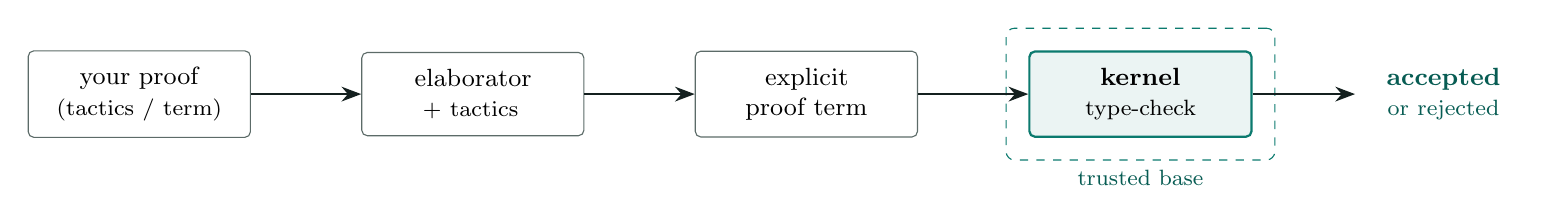
\begin{tikzpicture}[
  font=\small,
  box/.style={draw=muted, rounded corners=2pt, fill=white, inner sep=6pt,
    minimum height=9mm, align=center, text width=24mm},
  kbox/.style={draw=accent, line width=0.8pt, rounded corners=2pt,
    fill=accent!8, inner sep=6pt, minimum height=9mm, align=center,
    text width=24mm},
  flow/.style={-{Stealth[length=2.5mm]}, draw=ink, line width=0.7pt},
]
  \node[box] (src) {your proof\\{\footnotesize (tactics / term)}};
  \node[box, right=14mm of src] (elab) {elaborator\\{\footnotesize + tactics}};
  \node[box, right=14mm of elab] (term) {explicit\\proof term};
  \node[kbox, right=14mm of term] (kern) {\textbf{kernel}\\{\footnotesize type-check}};
  \node[right=13mm of kern, align=center, text width=20mm] (ok)
    {\color{accentdark}\textbf{accepted}\\{\footnotesize or rejected}};
  \draw[flow] (src) -- (elab);
  \draw[flow] (elab) -- (term);
  \draw[flow] (term) -- (kern);
  \draw[flow] (kern) -- (ok);
  \begin{scope}[on background layer]
    \node[draw=accent, dashed, rounded corners=3pt, inner sep=8pt,
      fit=(kern), label={[accentdark,font=\footnotesize]below:trusted base}] {};
  \end{scope}
\end{tikzpicture}%
}
\caption{How a proof is checked. Everything left of the dashed box may be
elaborate or buggy; soundness rests only on the kernel re-checking the final
term. Boxes are artifacts; solid arrows are transformations.}
\label{fig:pipeline}
\end{figure}

% ===========================================================================
\section{Situating Lean: TLA\texorpdfstring{\textsuperscript{+}}{+} and Haskell}\label{sec:situate}
% ===========================================================================
The fastest way to understand Lean is by contrast with tools answering
\emph{different} questions (\Cref{tab:compare}).

\paragraph{Versus TLA\textsuperscript{+}.} TLA\textsuperscript{+} is a
\emph{specification language}: you model a system---often concurrent or
distributed---as a state machine and state properties in temporal logic, then
check them primarily by \textbf{model checking}, in which the TLC checker
exhaustively explores a \emph{finite} state space and prints a counterexample
trace when a property fails. Lean does not explore states; it \textbf{proves}
statements deductively over possibly-infinite objects. The mental shift is
bounded-and-automatic-with-counterexamples (TLC) versus
unbounded-and-deductive-without-counterexamples (Lean). Lean's \code{#eval} and
\code{decide} can feel faintly model-checker-like on finite decidable
propositions, but that is evaluating a decision procedure, not exploring a
temporal state space. Reach for TLA\textsuperscript{+} to ask ``does my design
have a bad interleaving?''; reach for Lean to ask ``is this true for all inputs,
provably?''.

\paragraph{Versus Haskell.} Much will feel familiar: both are pure and
functional with type classes, algebraic data types, \code{do} notation, monads,
and strong inference. The differences are the point. Lean has full
\emph{dependent} types (\Cref{sub:fp}); it is total by default where Haskell is
lazy and partial (\code{undefined} inhabits every Haskell type); and its types
can state theorems, which Haskell's cannot in any practical sense. Treat Haskell
as good intuition for the syntax and the functional style, then add
``types can talk about values, and functions must terminate.''

\begin{table}[t]
\centering\small
\begin{tabular}{@{}p{2.5cm}p{3.5cm}p{4.3cm}p{3.2cm}@{}}
\toprule
 & \textbf{TLA\textsuperscript{+}} & \textbf{Lean 4} & \textbf{Haskell}\\
\midrule
Primary job & specify systems \& temporal behavior & prove theorems; write
verified programs & write programs\\[2pt]
How you check & model-check a \emph{finite} state space (TLC); finds
counterexamples & \emph{deduce} over infinite objects; no counterexamples unless
you search & type-check; run tests\\[2pt]
Types & untyped set theory & full \emph{dependent} types; can express theorems &
Hindley--Milner + extensions\\[2pt]
Totality & --- & total by default (termination-checked) & lazy \& partial\\[2pt]
Ask it & ``bad interleaving?'' & ``true for all inputs, provably?'' &
``elegant program?''\\
\bottomrule
\end{tabular}
\caption{Three overlapping but distinct questions. Lean is the deductive,
unbounded one.}
\label{tab:compare}
\end{table}

% ===========================================================================
\section{Is Lean a general-purpose language? IO, data, C interop}\label{sec:general}
% ===========================================================================
Yes. Lean~4 is a genuine general-purpose language, not a proof-only toy. It
compiles to C and then to native code, has an \code{IO} monad for real
input/output, ships arrays, hash maps, strings and \code{ByteArray} for ordinary
data manipulation, and is substantial enough that \emph{the Lean compiler and
much of its standard library are written in Lean itself}
\cite{demoura-lean4}. A minimal program:

\begin{lstlisting}
def main : IO Unit := do
  let stdin ← IO.getStdin
  let line ← stdin.getLine
  IO.println s!"you said: {line.trim}"        -- string interpolation
\end{lstlisting}

\noindent \textbf{Calling C from Lean.} The \code{@[extern "sym"]} attribute
binds a Lean declaration to an external C symbol; you give a Lean signature and
type-level model, and link the C implementation:

\begin{lstlisting}
@[extern "lean_sqrt"]        -- calls C function `double lean_sqrt(double)`
opaque cSqrt (x : Float) : Float
\end{lstlisting}

\noindent \textbf{Calling Lean from C.} The \code{@[export sym]} attribute
exposes a Lean function under an unmangled, C-callable name; you compile the Lean
code and link against the Lean runtime (\texttt{libleanshared}), which provides
garbage collection and the reference-counting discipline Lean's compiled objects
use:

\begin{lstlisting}
@[export my_add]             -- becomes C-callable `lean_object* my_add(...)`
def myAdd (a b : Nat) : Nat := a + b
\end{lstlisting}

\noindent So interoperation runs both directions. The one caveat is the runtime:
Lean-compiled code is C \emph{plus} the Lean runtime and its object model
(reference-counted \code{lean\_object*}, with each parameter either owned or
borrowed), so embedding Lean in a C program links a runtime rather
than dropping in a freestanding \code{.o} \cite{lean-ffi}. Lean is thus usable
for library building and data-processing tools; what it is \emph{not} is a
drop-in systems language with no runtime.

% ===========================================================================
\section{Tooling and editors}\label{sec:tooling}
% ===========================================================================
Lean~4 ships a \textbf{language server} (the \code{lean --server} command,
speaking the \emph{Language Server Protocol}, LSP), so editor support is a matter
of an LSP client plus a plugin that renders the \emph{infoview}---the live
display of the proof goal at the cursor.

\begin{itemize}[leftmargin=1.4em,itemsep=2pt]
  \item \textbf{VS Code} has the most complete, first-party extension. (Noted
    for completeness; a preference against it does not block anything below.)
  \item \textbf{Emacs} (\code{lean4-mode}) and \textbf{Neovim}
    (\code{lean.nvim}) are actively maintained LSP clients with infoview
    support---the mainstream non-VS-Code choices.
  \item \textbf{Xcode: there is no Lean plugin.} Xcode does not expose a
    general third-party-language / LSP extension point, and no Lean~4 Xcode
    integration exists as of 2026. If you want to stay in the Apple toolchain,
    the practical route is the command line (below) plus an LSP-capable editor
    (Emacs/Neovim) alongside it.
  \item \textbf{Command line only} is entirely viable, and is how the companion
    project is checked:
\end{itemize}

\begin{lstlisting}
lake build                        -- type-check the whole project = check all proofs
lake env lean Primer/Basics.lean  -- run one file, printing its #eval / #check output
\end{lstlisting}

\noindent There is no separate ``test'' step for the proofs: a clean
\code{lake build} \emph{is} the verification, because the build is exactly the
kernel checking every term (\Cref{sec:prover}). One practical caution learned
while assembling this primer: \code{lake build} can report success from a cached
build artifact; when you want the ground truth for a single file, run
\code{lake env lean <file>}, which re-elaborates from source.

% ===========================================================================
\section{The proof experience and the crypto-relevant layer}\label{sec:proofs}
% ===========================================================================
Proofs are written either in \emph{term mode} (hand Lean the term directly) or,
more often, in \emph{tactic mode}: a \code{by} block runs \textbf{tactics}---small
commands that transform the goal while Lean assembles the underlying term. In an
editor the infoview shows the evolving goal; on the command line you reason it
out. A working vocabulary: \code{rfl} (true by computation), \code{decide} (run a
decision procedure on a finite/decidable goal), \code{simp} (rewrite with a lemma
database), \code{omega} (linear arithmetic over integers and naturals), and
\code{induction}. \emph{Every} construct, tactic, and lemma used in this primer's
code is glossed in the reference (\Cref{app:reference}); reach for it whenever a
listing shows something unfamiliar.

Lean's \code{BitVec n} type---fixed-width machine words with wraparound
arithmetic---is the layer where cryptography lives, and it is directly relevant
to the companion survey of SHA-256 formalization. SHA-256's whole primitive layer
is a few total functions:

\begin{lstlisting}
def rotr (x : BitVec 32) (n : Nat) : BitVec 32 := (x >>> n) ||| (x <<< (32 - n))
def Ch     (x y z : BitVec 32) := (x &&& y) ^^^ ((~~~x) &&& z)
def Maj    (x y z : BitVec 32) := (x &&& y) ^^^ (x &&& z) ^^^ (y &&& z)
def Sigma0 (x : BitVec 32) := rotr x 2 ^^^ rotr x 13 ^^^ rotr x 22

-- Over ALL 256 eight-bit words, brute force (`decide`) settles this identity:
example : ∀ x : BitVec 8, x ^^^ x = 0#8 := by decide
-- Over 32 bits it is 2³² cases; there `decide` is hopeless and the tactic is
-- `bv_decide` — bit-blast to SAT and check an LRAT certificate in-kernel.
\end{lstlisting}

\noindent That last tactic, \code{bv\_decide}, is verified bit-blasting: it hands
the goal to a SAT solver and then re-checks the solver's refutation certificate
with a Lean-verified checker, so the untrusted solver never enters the trusted
base \cite{boving-bvdecide}. It is why Lean is now a strong platform for
bit-level cryptographic reasoning even though a full software SHA-256 correctness
proof in Lean does not yet exist---the subject of the companion survey.

% ===========================================================================
\section{Verifying properties of your own code}\label{sec:verify}
% ===========================================================================
Set expectations precisely. Lean is excellent for proving properties of
\emph{pure functions}, data-structure \emph{invariants}, and math-heavy
\emph{kernels} that you model or re-implement in Lean; there you can prove a
statement for \emph{all} inputs. Lean is \emph{not} a push-button verifier for an
arbitrary existing Rust, Python, or C repository---that is the domain of
SMT-backed tools (\emph{Satisfiability Modulo Theories}: automatic decision
procedures over arithmetic, arrays, and the like) such as Dafny or Why3, or of
model checkers such as TLA\textsuperscript{+}. The productive loop is: model the
critical pure core in Lean, prove it there, and treat that as your trustworthy
reference. A representative shape---a fast implementation proved equal to an
obvious reference model:

\begin{lstlisting}
def sumTo : Nat → Nat                        -- reference model
  | 0 => 0
  | n + 1 => (n + 1) + sumTo n

def sumToAcc : Nat → Nat → Nat               -- optimized tail-recursive version
  | 0,     acc => acc
  | n + 1, acc => sumToAcc n (acc + (n + 1))

theorem sumTo_correct (n : Nat) : sumToAcc n 0 = sumTo n := by
  simp [sumToAcc_eq]                         -- via a generalized accumulator lemma
\end{lstlisting}

% ===========================================================================
\section{A worked theorem: the Josephus closed form}\label{sec:josephus}
% ===========================================================================
To show a non-trivial result carried all the way to a machine-checked proof, we
formalize a classic from Knuth's \emph{Concrete Mathematics}
\cite{concrete-math}: the Josephus problem. Of $n$ people in a circle every
second is eliminated; the survivor's position $J(n)$ satisfies
\[
  J(1)=1,\qquad J(2n)=2J(n)-1,\qquad J(2n+1)=2J(n)+1,
\]
with the memorable closed form: writing $n = 2^m + \ell$ with $0 \le \ell < 2^m$,
\[
  \boxed{\,J(2^m+\ell) = 2\ell+1\,}
\]
equivalently ``$J(n)$ is the binary numeral of $n$ rotated left by one bit''
(e.g.\ $13 = 1101_2 \mapsto 1011_2 = 11 = J(13)$). The bit-rotation reading is a
direct callback to \code{rotr} in \Cref{sec:proofs}, which is why this problem is
pleasantly close to the SHA-256 world. Here is the recurrence and the general
theorem, both machine-checked in pure Lean (no library). The listing below is
\textbf{what you type}---the definition and a tactic proof; any construct in it
is glossed in \Cref{app:reference}:

\begin{lstlisting}
def josephus : Nat → Nat
  | 0 => 0
  | 1 => 1
  | n + 2 =>
      have : (n + 2) / 2 < n + 2 := Nat.div_lt_self (by omega) (by omega)
      if (n + 2) % 2 = 0 then 2 * josephus ((n + 2) / 2) - 1
                         else 2 * josephus ((n + 2) / 2) + 1

theorem josephus_pow (m : Nat) :
    ∀ l, l < 2 ^ m → josephus (2 ^ m + l) = 2 * l + 1 := by
  induction m with
  | zero => intro l hl; rw [Nat.pow_zero] at hl ⊢; have : l = 0 := by omega
            subst this; simp [josephus]
  | succ m ih =>
      intro l hl
      have hpow : (2 : Nat) ^ (m + 1) = 2 * 2 ^ m := by rw [Nat.pow_succ]; omega
      have hpos : 0 < (2 : Nat) ^ m := Nat.two_pow_pos m
      rcases (show l % 2 = 0 ∨ l % 2 = 1 by omega) with hpar | hpar
      · have hjm : l / 2 < 2 ^ m := by omega
        have hk : (2:Nat) ^ (m+1) + l = 2 * (2 ^ m + l / 2) := by omega
        rw [hk, josephus_even (2 ^ m + l / 2) (by omega), ih (l / 2) hjm]; omega
      · have hjm : l / 2 < 2 ^ m := by omega
        have hk : (2:Nat) ^ (m+1) + l = 2 * (2 ^ m + l / 2) + 1 := by omega
        rw [hk, josephus_odd (2 ^ m + l / 2) (by omega), ih (l / 2) hjm]; omega
\end{lstlisting}

\noindent Everything after \code{:= by} is a script of \emph{tactics}---your
instructions for building the proof, not the proof itself. \textbf{What Lean
generates} from it is an ordinary term, which is what the kernel actually
checks. Printing it (\code{\#print josephus\_pow}, trimmed here) shows the
\code{induction} tactic became an application of \code{Nat}'s recursor, with your
two cases as its arguments:

\begin{lstlisting}
-- WHAT LEAN GENERATES (the proof term the kernel checks) — abbreviated:
theorem josephus_pow : ∀ (m l : Nat), l < 2 ^ m → josephus (2 ^ m + l) = 2*l + 1 :=
fun m =>
  Nat.recAux
    (fun l hl => …)          -- the m = 0 case you wrote as `| zero => …`
    (fun m ih l hl => …)     -- the m+1 case you wrote as `| succ m ih => …`
    m
-- (the real term fills each `…` with ~15 lines of Eq.mpr/congrArg/… plumbing)
\end{lstlisting}

\noindent You never write that term by hand---that is the whole point of tactic
mode. But it exists, and the kernel re-checks it; the tactics are only a
convenient way to produce it. The proof itself is a textbook induction on $m$
that splits on the parity of $\ell$ and steps down through the recurrence---exactly
the \emph{Concrete Mathematics} argument, now checked by the kernel rather than
by a careful reader.
The full file also machine-checks (over $1 \le n \le 2000$, via
\code{native\_decide}) that the recurrence, the closed form, and the
one-bit-rotation form agree. This is the kind of concrete, self-contained result
that Lean makes routine---and, notably, it required no mathematics library at
all.

% ===========================================================================
\section{Illuminating examples: discrete probability}\label{sec:prob}
% ===========================================================================
Probability makes a nice showcase because the surprising facts become things the
machine can \emph{check}. Over a finite, equally-likely sample space a
probability is just \code{favorable / total} (two naturals), and a claim
``$p > 1/2$'' is the exact inequality \code{2 * favorable > total}---no real
numbers required.

\paragraph{Monty Hall.} Enumerate the nine equally-likely \code{(car, firstPick)}
games. After the host opens a goat door, switching wins \emph{exactly when your
first pick was wrong}, so it wins $6/9 = 2/3$ against staying's $3/9$:

\begin{lstlisting}
def games : List (Nat × Nat) :=            -- all 9 (car, pick) pairs
  [0,1,2].flatMap (fun car => [0,1,2].map (fun pick => (car, pick)))

def countWhere (xs : List α) (p : α → Bool) : Nat := (xs.filter p).length

example : games.length = 9
        ∧ countWhere games (fun g => g.1 == g.2) = 3       -- staying wins
        ∧ countWhere games (fun g => g.1 != g.2) = 6 := by  -- switching wins
  decide
\end{lstlisting}

\paragraph{The birthday paradox.} Among $n$ people (365 equally-likely
birthdays), all differ with probability $\bigl(\prod_{i<n}(365-i)\bigr)/365^{\,n}$;
a shared birthday becomes more likely than not once \code{2 * numerator < 365^n}.
The numbers are $\sim$60 digits, so \code{native_decide}---which \emph{compiles}
the check to native code rather than reducing it in the kernel---does the
arithmetic (Lean's \code{Nat} is arbitrary-precision). It confirms the threshold
is \emph{exactly} 23 people:

\begin{lstlisting}
def noCollisionNum : Nat → Nat
  | 0 => 1
  | n + 1 => (365 - n) * noCollisionNum n

theorem birthday_threshold :
    2 * noCollisionNum 23 < 365 ^ 23 ∧ 2 * noCollisionNum 22 ≥ 365 ^ 22 := by
  native_decide
\end{lstlisting}

\noindent The companion \code{Primer/Probability.lean} adds De M\'er\'e's 1654
dice problem---the wager that launched the subject---machine-checking that a bet
paying off on ``one 6 in four rolls'' clears $1/2$ while ``one double-6 in
twenty-four rolls'' falls just short. Every construct these listings use is
glossed in \Cref{app:reference}.

% ===========================================================================
\section{mathlib, and where to go next}\label{sec:next}
% ===========================================================================
\textbf{mathlib} is the community's large, coherent library of formalized
mathematics---algebra through analysis and beyond---with the lemmas and
automation to match \cite{avigad-mil}. It is what you pull in when a proof rests
on real mathematics; it is also a heavy dependency (its prebuilt object cache is
several gigabytes, and the first \code{import Mathlib} takes minutes). Everything
in this primer \emph{deliberately} uses none of it---core Lean plus its standard
library, \emph{Batteries}, is enough for algorithmic and bit-level work, and the
project stays instant and offline. That is a choice, not a limitation: when a
proof genuinely needs mathematics, you add \verb|require mathlib| to your
\texttt{lakefile}, run \verb|lake exe cache get| to fetch the prebuilt library,
and its full power is available.

\paragraph{What it buys you.} The companion \texttt{mathlib-tour/} project makes
the trade-off concrete. The one awkward step in \Cref{sec:prover}---proving
$(k{+}1)^2 = k^2 + 2k + 1$ by hand with \code{simp only [Nat.succ\_mul,
Nat.mul\_succ]; omega}---collapses to a single \code{ring}. It also states things
core Lean cannot: an actual finite sum $\sum_{i<n}(2i+1) = n^2$, the irrationality
of $\sqrt 2$, and dice probability as a genuine rational over a \code{Finset}
rather than the integer counting the primer used to stay library-free.

\paragraph{Where to go next.} \emph{Theorem Proving in Lean~4}
\cite{avigad-tpil4} for the proof language, \emph{Functional Programming in Lean}
\cite{christiansen-fpil} for the programming side, and \emph{Mathematics in Lean}
\cite{avigad-mil} for working with mathlib. The companion \texttt{primer/} project
holds every core-Lean example above as runnable, type-checked source, and
\texttt{mathlib-tour/} holds the mathlib ones.

% ---------------------------------------------------------------------------
\section*{Glossary}
\addcontentsline{toc}{section}{Glossary}
\begin{description}[leftmargin=0pt,style=nextline,itemsep=1pt]
  \item[Kernel] the small trusted core that checks a term has its claimed type;
    the sole component that must be trusted for soundness.
  \item[Term / Proposition] a term is a value/program; a proposition is a
    statement realized as a type whose terms are its proofs (Curry--Howard).
  \item[Tactic] a command that transforms the proof goal, building a proof term
    (e.g.\ \code{simp}, \code{omega}, \code{induction}).
  \item[Dependent type] a type that mentions a value (e.g.\ length-indexed
    vectors); what lets types state theorems.
  \item[ITP / ATP] interactive theorem prover (human-guided, machine-checked)
    versus automated theorem prover (search-driven).
  \item[LSP / FFI] Language Server Protocol (editor integration); Foreign
    Function Interface (calling between languages, here Lean$\leftrightarrow$C).
  \item[\texttt{decide} / \texttt{bv\_decide}] run a decision procedure on a
    decidable goal; the latter bit-blasts \texttt{BitVec} goals to a SAT solver
    and re-checks its certificate.
  \item[\texttt{elan} / \texttt{lake}] the toolchain manager (installs/selects Lean versions) and
    the build system / package manager.
\end{description}

% ===========================================================================
\appendix
\section{Syntax and tactics reference}\label{app:reference}
% ===========================================================================
Every language construct used in this primer's code listings, grouped and
glossed. ``Tactics'' run inside a \code{by} block; ``commands'' (starting with
\code{\#}) run at compile time and print to the infoview.

\newcommand{\grp}[1]{\medskip\noindent\textbf{#1}\nopagebreak\par\nobreak\smallskip}

\grp{Commands and declarations.}
\begin{tabular}{@{}l@{\hspace{1.4em}}p{9cm}@{}}
\verb|#eval e| & run \texttt{e} and print the result \\[1.5pt]
\verb|#check e| & print the type of \texttt{e} without running it \\[1.5pt]
\verb|#print n| & print the definition or proof term of \texttt{n} \\[1.5pt]
\verb|def| & define a value or function \\[1.5pt]
\verb|theorem| / \verb|example| & state (and prove) a proposition; \texttt{example} is unnamed \\[1.5pt]
\verb|inductive ... where| & declare an algebraic data type by its constructors \\[1.5pt]
\verb|opaque| & declare a value with no body (e.g.\ one supplied externally) \\[1.5pt]
\verb|@[extern "sym"]| & implement this declaration with the C symbol \texttt{sym} \\[1.5pt]
\verb|@[export sym]| & expose this declaration to C under the name \texttt{sym} \\
\end{tabular}

\grp{Expression syntax.}
\begin{tabular}{@{}l@{\hspace{1.4em}}p{9cm}@{}}
\verb|fun x => e| & anonymous function (lambda) \\[1.5pt]
\verb|let x := e| / \verb|let x <- e| & local binding; the \verb|<-| form sequences a monadic (e.g.\ \texttt{IO}) step \\[1.5pt]
\verb|do ...| & sequence monadic actions \\[1.5pt]
\verb|if c then a else b| & conditional \\[1.5pt]
\verb!| pat => e! & a pattern-match arm (in a \texttt{def} or \texttt{match}) \\[1.5pt]
\verb|(a, b)|, \verb|p.1|, \verb|p.2| & a pair and its two projections \\[1.5pt]
\verb|s!"... {x} ..."| & string interpolation \\[1.5pt]
\verb|0#8|, \verb|0xff#32| & a \texttt{BitVec} literal, written \emph{value}\texttt{\#}\emph{width} \\[1.5pt]
\verb|:| \ / \ \verb|:=| & type ascription \ / \ ``is defined as'' \\
\end{tabular}

\grp{Operators.}
\begin{tabular}{@{}l@{\hspace{1.4em}}p{9cm}@{}}
\verb|+  -  *  /  %| & arithmetic on \texttt{Nat} (\texttt{/} and \texttt{\%} are truncating) \\[1.5pt]
\verb|^| & exponentiation \\[1.5pt]
\verb|=  <  <=  >=| & (in)equality \emph{propositions}; \verb|==| and \verb|!=| are Boolean \\[1.5pt]
\verb!&&&  |||  ^^^  ~~~! & bitwise and / or / xor / not on \texttt{BitVec} \\[1.5pt]
\verb|>>>  <<<| & right / left shift on \texttt{BitVec} \\
\end{tabular}

\grp{Tactics.}
\begin{tabular}{@{}l@{\hspace{1.4em}}p{9cm}@{}}
\verb|rfl| & close a goal whose two sides compute to the same value \\[1.5pt]
\verb|decide| & decide a decidable goal by evaluating it \\[1.5pt]
\verb|native_decide| & like \texttt{decide}, but compiled to native code (large computations) \\[1.5pt]
\verb|simp| / \verb|simp only [ls]| & simplify by rewriting (with \emph{only} the lemmas \texttt{ls}) \\[1.5pt]
\verb|omega| & decide linear arithmetic over \texttt{Nat}/\texttt{Int} \\[1.5pt]
\verb|induction n with ...| & induct on \texttt{n}, one arm per constructor; an arm binds the induction hypothesis \\[1.5pt]
\verb|intro h| & move a \verb|forall|/\verb|->| premise into the context \\[1.5pt]
\verb|rw [eqs]| & rewrite the goal with equations; \verb|rw [e] at h |\(\vdash\) also targets \texttt{h} and the goal \\[1.5pt]
\verb|subst h| & eliminate a variable using an equation hypothesis \\[1.5pt]
\verb|have h : P := pf| & introduce a proved sub-fact \texttt{h} \\[1.5pt]
\verb|show P| & restate the goal in a definitionally-equal form \\[1.5pt]
\verb|calc a = b := ...| & a chain of (in)equalities, each with its justification \\[1.5pt]
\verb!rcases e with h | h! & case-split on a disjunction or structure \\[1.5pt]
\verb|·| & focus the first remaining goal (one bullet per case) \\
\end{tabular}

\paragraph{Referenced library items.} Their names describe them:
\texttt{Nat.recAux} (the recursor / induction principle for \texttt{Nat}),
\texttt{Eq.refl a} (the proof \texttt{a = a}), the arithmetic lemmas
\texttt{Nat.succ\_mul}, \texttt{Nat.mul\_succ}, \texttt{Nat.pow\_zero},
\texttt{Nat.pow\_succ}, \texttt{Nat.two\_pow\_pos}, \texttt{Nat.div\_lt\_self};
the list operations \texttt{List.map}, \texttt{List.filter},
\texttt{List.flatMap}, \texttt{List.range}, \texttt{.length}; and
\texttt{Vector.append} (length-tracking concatenation). The unfolding equation of
a well-founded definition \texttt{f} is available as \texttt{f.eq\_def}.

\printbibliography[heading=bibintoc,title={References}]

\end{document}
